% Intended LaTeX compiler: pdflatex
\documentclass[11pt]{article}
\usepackage[utf8]{inputenc}
\usepackage[T1]{fontenc}
\usepackage{graphicx}
\usepackage{longtable}
\usepackage{wrapfig}
\usepackage{rotating}
\usepackage[normalem]{ulem}
\usepackage{amsmath}
\usepackage{amssymb}
\usepackage{capt-of}
\usepackage{hyperref}
\usepackage{booktabs}
\usepackage{import}
\usepackage[LGR, T1]{fontenc}
\usepackage[greek, english, american]{babel}
\usepackage{alphabeta}
\usepackage{esint}
\usepackage{mathtools}
\usepackage{esdiff}
\usepackage{makeidx}
\usepackage{glossaries}
\usepackage{newfloat}
\usepackage{minted}
\usepackage[a4paper, margin=3cm]{geometry}
\usepackage{chemfig}
\usepackage{svg}
\renewcommand{\tablename}{Πίνακας}
\author{Βιδιάνος Γιαννίτσης}
\date{\today}
\title{Progress Report για την Αναερόβια Χώνευση Υδρολυμένων Υπολειμμάτων Τροφών}
\hypersetup{
 pdfauthor={Βιδιάνος Γιαννίτσης},
 pdftitle={Progress Report για την Αναερόβια Χώνευση Υδρολυμένων Υπολειμμάτων Τροφών},
 pdfkeywords={},
 pdfsubject={},
 pdfcreator={Emacs 29.3 (Org mode 9.6.15)}, 
 pdflang={English}}
\makeatletter
\newcommand{\citeprocitem}[2]{\hyper@linkstart{cite}{citeproc_bib_item_#1}#2\hyper@linkend}
\makeatother

\usepackage[notquote]{hanging}
\begin{document}

\maketitle

\subsection{Περιεχόμενα}
\label{sec:orgbb94266}

\section{Θεωρητικό Υπόβαθρο}
\label{sec:org57e70ec}
\subsection{Σκοπός}
\label{sec:org6c86760}
Σκοπός της διπλωματικής είναι η επεξεργασία υπολειμμάτων τροφών. Αρχικά έγινε υδρόλυση με ένα εμπορικό σκεύασμα που περιέχει ένζυμα και μικροοργανισμούς (μιξ) για διαλυτοποίηση της οργανικής ύλης και μετέπειτα αναερόβια χώνευση του υδρολύματος για παραγωγή μεθανίου.

\subsection{Παράγοντες που επηρεάζουν την διεργασία}
\label{sec:org3243f22}
\begin{itemize}
\item {\color{blue} \textbf{Ποσότητα Μιξ} }

\item {\color{blue} \textbf{Θερμοκρασία} }

\item {\color{blue}pH}
\end{itemize}

\begin{itemize}
\item {\color{orange}Αερισμός}

\item {\color{orange} \textbf{Αραίωση Δείγματος} }

\item {\color{orange} \textbf{Ανάδευση} }
\end{itemize}

Επιλέχθηκαν οι τιμές 35 και 40 \(^oC\) για τα πειράματα ως ενδεικτικές τιμές θερμοκρασίας στη θερμόφιλη περιοχή. Μία αρχική δοκιμή είχε γίνει και στους 45 \(^oC\).

\begin{table}[htbp]
\caption{Προετοιμασία Δειγμάτων για Υδρόλυση}
\centering
\begin{tabular}{lrrrrr}
Μιξ (ml) & 0 & 1 & 2 & 4 & 8\\[0pt]
Food Waste (g) & 200 & 200 & 200 & 200 & 200\\[0pt]
Νερό (ml) & 600 & 600 & 600 & 600 & 600\\[0pt]
\end{tabular}
\end{table}

Η ανάδευση ρυθμίστηκε στα 120 rpm με βάση προηγούμενα πειράματα

\section{Αποτελέσματα από τα πειράματα υδρόλυσης}
\label{sec:org4df776a}
\subsection{Κατανομή Προιόντων}
\label{sec:org32396b0}
Ένα από τα βασικά κριτήρια για να κρίνουμε την διεργασία είναι τα παραγόμενα προιόντα (είτε ως σύνολο ή ξεχωριστά για το κάθε προιόν).

\begin{center}
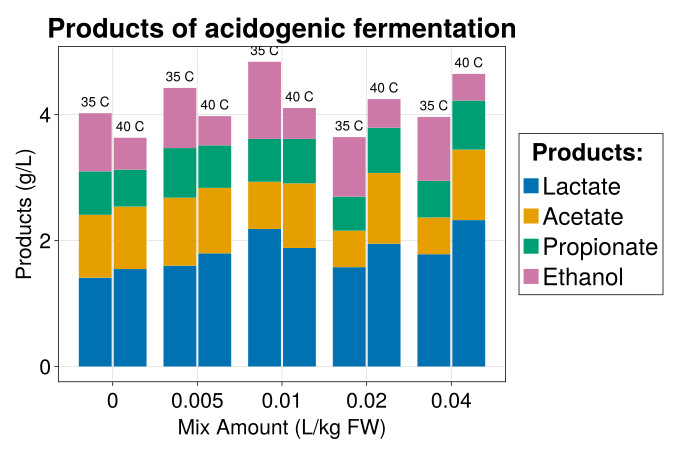
\includegraphics[width=.9\linewidth]{../plots/35_40_comp/final_products.png}
\end{center}

\subsection{Συγκεντρωτικά Κριτήρια}
\label{sec:org8646fa4}
Πολύ συχνά, αντί να ασχοληθούμε όμως με την κατανομή των προιόντων, κοιτάμε κάποια συγκεντρωτικά κριτήρια για αυτά.

\begin{center}
\includegraphics[width=.9\linewidth]{../plots/35_40_comp/acidification_comp.png}
\end{center}

\begin{center}
\includegraphics[width=.9\linewidth]{../plots/35_40_comp/Δprod.png}
\end{center}

\subsection{Ανάλυση Ευαισθησίας}
\label{sec:org6c30cd9}
Ως ένα τελευταίο αποτέλεσμα, παρουσιάζεται μία ανάλυση ευαισθησίας.
\begin{center}
\includegraphics[width=.9\linewidth]{../plots/sensitivity/global_tornado.png}
\end{center}

Από αυτήν βλέπουμε πως η αύξηση της θερμοκρασίας βοηθάει στην παραγωγή τριών από τα 4 προιόντα, οπότε, αν δεν μας ενδιαφέρει πολύ η αιθανόλη, η υψηλή θερμοκρασία (40 \(^oC\)) είναι η πιο επιθυμητή.

Μάλιστα, αν περιορίσουμε την ευαισθησία ώστε να είναι καθαρά στην ποσότητα μιξ ανά θερμοκρασία, βλέπουμε ότι στους 35 \(^oC\), το οξικό έχει μία μεγάλη τάση μείωσης όσο προσθέτουμε το μιξ. Αυτός είναι και ο βασικότερος λόγος να προτιμηθεί η θερμοκρασία 40 \(^oC\). Επίσης φαίνεται πως εκεί, τα τρία προιόντα που θα παραχθούν έχουν θετική ευαισθησία προς την ποσότητα μιξ.

\begin{center}
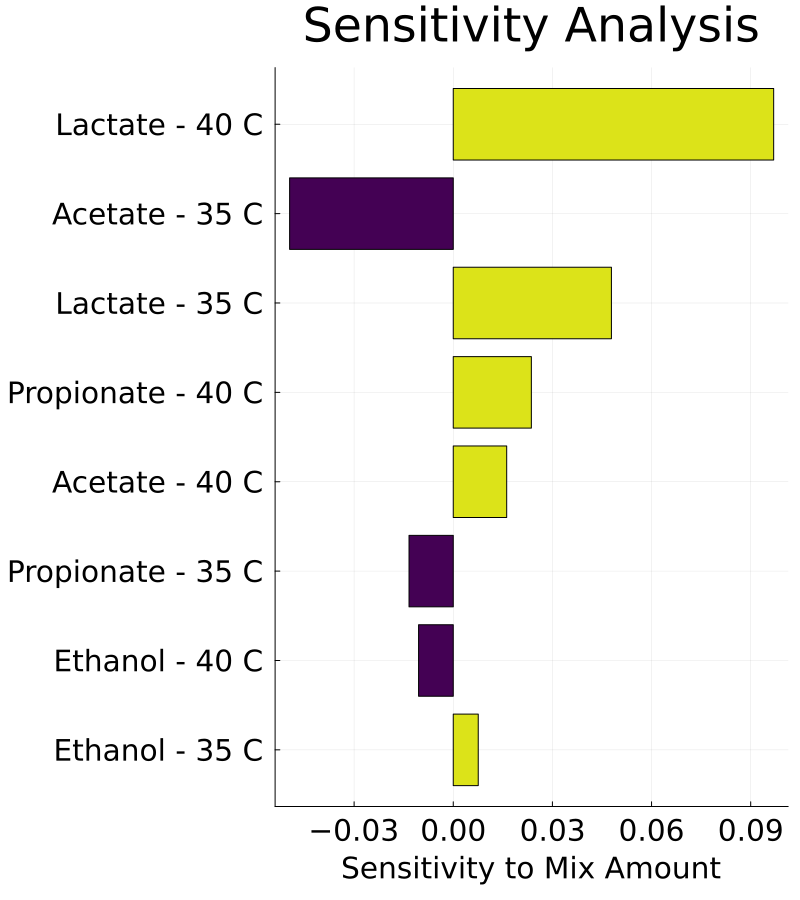
\includegraphics[width=.9\linewidth]{../plots/sensitivity/temperature_tornado.png}
\end{center}

Όμως, αν περιορίσουμε τις ποσότητες μιξ στα 2-8 ml, βλέπουμε πως αυτή η θετική ευαισθησία έχει πρακτικά χαθεί, οπότε πιθανότατα δεν έχει νόημα να πάμε πάνω από 2 ml.
\begin{center}
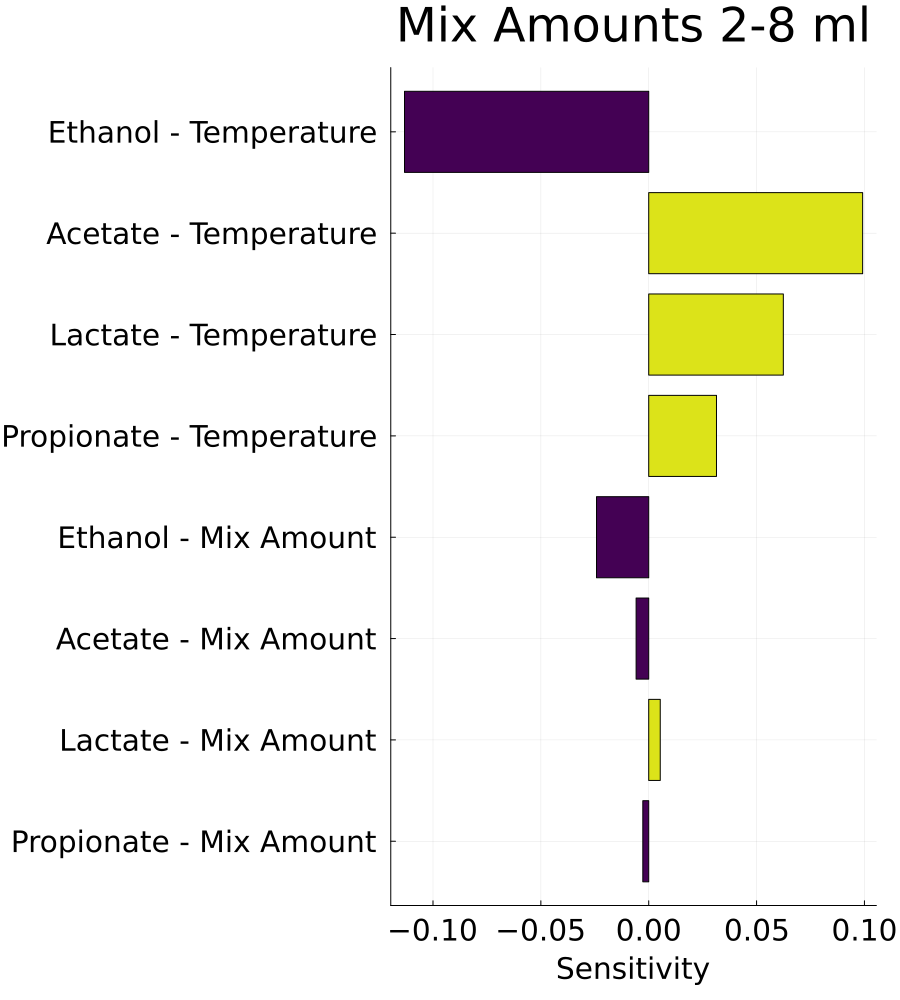
\includegraphics[width=.9\linewidth]{../plots/sensitivity/tornado_high.png}
\end{center}

\section{Συμπεράσματα}
\label{sec:orgeb76f50}
Καταλήγουμε πως η θερμοκρασία 40 \(^oC\) είναι καλύτερη και ότι οι πολύ υψηλές ποσότητες μιξ είναι πολύ πιθανό να μην βοηθάνε την διεργασία. Οπότε για την χώνευση προετοιμάστηκε υπόστρωμα από υδρόλυση στους 40 \(^oC\) με ποσότητες μιξ 0, 1, 2 και 4 ml. 

\section{Προετοιμασία υποστρώματος για χώνευση}
\label{sec:orgffdda6e}
Για να τρέξουμε την αναερόβια χώνευση, προετοιμάσαμε καινούργια υδρολύματα καθώς τα προηγούμενα δεν είχαν αποθηκευτεί. Σε αυτά έχουν μετρηθεί TS, VS, sCOD και tCOD.
\begin{center}
\includegraphics[width=.9\linewidth]{../plots/26_03/complete_cod_bar_26_03.png}
\end{center}

\begin{center}
\includegraphics[width=.9\linewidth]{../plots/26_03/ts_vs_bar_plot_26_03.png}
\end{center}

\section{Πειραματική Διαδικασία Αναερόβιας Χώνευσης}
\label{sec:orgf4196f1}
\subsection{Πειραματική Διάταξη}
\label{sec:org51c0b6c}
\begin{center}
\includegraphics[width=.9\linewidth]{IMG_20240327_185818.jpg}
\end{center}

\subsection{Πειραματική Διαδικασία}
\label{sec:org85c27fc}
Στον πρώτο κύκλο πειραμάτων, προσθέσαμε 125 g λάσπης (1.55 g VS) και 315 g νερό με σκοπό μόλις προστεθεί το υδρόλυμα ο αντιδραστήρας να έχει πληρωθεί. Όλες οι τροφοδοσίες έγιναν με 100 mg sCOD-eq. Αρχικά, έγινε τροφοδοσία με οξικό, το οποίο ενεργοποιεί την λάσπη και μας δείχνει την μέγιστη δυνατή παραγωγή μεθανίου που μπορούμε να περιμένουμε από την λάσπη αυτή. Έπειτα, τροφοδοτήσαμε με τα υδρολύματα για να δούμε πόσο μεθάνιο θα παράγουν αυτά.

\subsection{Χαρακτηριστικά λάσπης}
\label{sec:org7ad0055}
\begin{table}[htbp]
\caption{Χαρακτηριστικά Λάσπης}
\centering
\begin{tabular}{lr}
Χαρακτηριστικό & Τιμή\\[0pt]
\hline
TS (g/l) & 46.28\\[0pt]
VS (g/l) & 12.36\\[0pt]
VS/TS & 0.267\\[0pt]
pH & 8.33\\[0pt]
Αλκαλικότητα (mg CaCO\textsubscript{3}/L) & 12250\\[0pt]
\end{tabular}
\end{table}

\subsection{Μοντέλο Gompertz για κινητική ανάλυση}
\label{sec:org06fdcd1}
Ένα από τα καλύτερα μοντέλα για κινητική ανάλυση αναερόβιας χώνευσης στη βιβλιογραφία είναι το τροποποιημένο μοντέλο Gompertz. Συνήθως προσαρμόζεται σε δεδομένα όγκου μεθανίου ανά g VS λάσπης ή όγκου μεθανίου ανά g COD που καταναλώνεται για σύγκριση με άλλες μελέτες.

\[ P(t) = P_{\max } \exp \left( - \exp \left[ \frac{R_{\max }e (λ-t)}{P_{\max }} + 1 \right] \right) \]

\section{Αποτελέσματα πρώτου κύκλου με υδρολύματα}
\label{sec:org11c1de9}
Δεν θα αναφερθούν πολύ αναλυτικά αποτελέσματα για τον κύκλο αυτόν λόγω των προβλημάτων που είχε. Οπότε, κάποιες τάσεις που φαίνονται εδώ πιθανόν να είναι σωστές, αλλά δεν είναι έμπιστο πείραμα και για αυτό έγινε και μία επανάληψη.

\begin{center}
\includegraphics[width=.9\linewidth]{../plots/BMPs/Hydrolyzed FW/methane_kinetics_hydrolysate_0_s1_r1_min.png}
\end{center}

\begin{center}
\includegraphics[width=.9\linewidth]{../plots/BMPs/Hydrolyzed FW/methane_kinetics_hydrolysate_0_s1_r1_hour.png}
\end{center}

\subsection{Untreated FW}
\label{sec:orgdc1293a}
Ένα από αυτά τα δείγματα (αυτό που τροφοδοτήθηκε με ακατέργαστο FW) δεν παρουσίασε αυτό το φαινόμενο και παρήγαγε πάρα πολύ λίγο μεθάνιο. Υποτέθηκε ότι μπορεί να υπήρξε κάποια διαρροή στο δείγμα αυτό.

\begin{center}
\includegraphics[width=.9\linewidth]{../plots/BMPs/Untreated FW/methane_kinetics_untreated_fw_s1_r1_hour.png}
\end{center}

\section{Αποτελέσματα δεύτερου κύκλου με υδρολύματα}
\label{sec:orgcbd04dc}

\subsection{Δείγμα 0}
\label{sec:orgbc641fe}
Τελικό pH = 8.93

\begin{center}
\includegraphics[width=.9\linewidth]{../plots/BMPs/Hydrolyzed FW/methane_kinetics_hydrolysate_0_s1_r2_hour.png}
\end{center}

\begin{center}
\includegraphics[width=.9\linewidth]{../plots/BMPs/Acetate/methane_kinetics_acet_test_0_s1_min.png}
\end{center}

\subsection{Δείγμα 1}
\label{sec:orgbc2ae3d}
Τελικό pH = 7.76

\begin{center}
\includegraphics[width=.9\linewidth]{../plots/BMPs/Hydrolyzed FW/methane_kinetics_hydrolysate_1_s1_r2_hour.png}
\end{center}

\begin{center}
\includegraphics[width=.9\linewidth]{../plots/BMPs/Acetate/methane_kinetics_acet_test_1_s1_min.png}
\end{center}

\subsection{Δείγμα 2}
\label{sec:org404c9f3}
Τελικό pH 7.19

\begin{center}
\includegraphics[width=.9\linewidth]{../plots/BMPs/Hydrolyzed FW/methane_kinetics_hydrolysate_2_s1_r2_hour.png}
\end{center}

\begin{center}
\includegraphics[width=.9\linewidth]{../plots/BMPs/Acetate/methane_kinetics_acet_test_2_s1_min.png}
\end{center}

\subsection{Δείγμα 4}
\label{sec:org1c9e04f}
Τελικό pH 6.76

\begin{center}
\includegraphics[width=.9\linewidth]{../plots/BMPs/Acetate/methane_kinetics_acet_test_4_s1_min.png}
\end{center}

\begin{center}
\includegraphics[width=.9\linewidth]{../plots/BMPs/Hydrolyzed FW/methane_kinetics_hydrolysate_4_s1_r2_hour.png}
\end{center}

\subsection{Untreated FW}
\label{sec:orgbe5def1}
Τελικό pH = 4.22

\begin{center}
\includegraphics[width=.9\linewidth]{../plots/BMPs/Untreated FW/methane_kinetics_untreated_fw_s1_r2_hour.png}
\end{center}

\begin{center}
\includegraphics[width=.9\linewidth]{../plots/BMPs/Acetate/methane_kinetics_acet_test_fw_s1_min.png}
\end{center}

Λογικά το πολύ όξινο αυτό pH είναι και ο λόγος για την χαμηλή παραγωγικότητα του δείγματος αυτού. Άρα φαίνεται πως η χώνευση ανεπεξεργαστού FW είναι ασταθείς και μπορεί να οδηγήσει σε κατάρρευση.

\section{Συγκριτικά αποτελέσματα αναερόβιας χώνευσης}
\label{sec:org2605ba7}
\subsection{Βιοχημικό Δυναμικό Μεθανίου (BMP)}
\label{sec:orgd4b96ef}
\begin{center}
\includegraphics[width=.9\linewidth]{../plots/BMPs/Hydrolyzed FW/acet_vs_hydro_bmp_s1_r2.png}
\end{center}

\subsection{Ρυθμός Παραγωγής Μεθανίου}
\label{sec:orga5eac0c}
Μονάδες: R\textsubscript{max} [=] \(\frac{\text{ml CH$_4$}}{hour}\) και SMA [=] \(\frac{\text{ml CH$_4$}}{\text{day} \cdot \text{g VS}}\).

\begin{center}
\begin{tabular}{lrrrr}
Sample\textsubscript{Name} & R\textsubscript{max} Acetate & R\textsubscript{max} Hydrolysate & SMA Acetate & SMA Hydrolysate\\[0pt]
\hline
Sample 0 & 459.84 & 0.043 & 7119.36 & 0.672\\[0pt]
Sample 1 & 326.88 & 0.108 & 5061.6 & 1.728\\[0pt]
Sample 2 & 374.04 & 0.114 & 5676.48 & 1.776\\[0pt]
Sample 4 & 579.0 & 0.08 & 8965.44 & 1.224\\[0pt]
Sample FW & 294.06 & 0.054 & 4554.72 & 0.84\\[0pt]
\end{tabular}
\end{center}

\subsection{Συμπεράσματα}
\label{sec:org01b2a23}
Βλέπουμε πως το περισσότερο μεθάνιο έχει παραχθεί από το υδρόλυμα με 1 ml μιξ και το δεύτερο καλύτερο είναι αυτό με τα 2 ml. Ακόμη, το 1 και το 2 έχουν πολύ κοντινό μέγιστο ρυθμό ανάπτυξης. Το υδρόλυμα με προσθήκη 2 ml μιξ όμως έχει μηδενικό lag time σε αντίθεση με το 1 ml, το οποίο είχε ένα lag time 4.5 ωρών. Συμπέρασμα του κύκλου αυτού είναι πως η καλύτερη απόδοση ήταν αυτή του υδρολύματος με προσθήκη 1 ml μιξ, ενώ αυτό με 2 ml είναι επίσης πολύ καλό.

Επίσης, τα δείγματα ανεπεξέργαστου FW και χωρίς προσθήκη του μιξ είχαν την χειρότερη απόδοση, το οποίο δείχνει πως η συνδυασμένη επίδραση της ρύθμισης της θερμοκρασίας και της προσθήκης του μιξ ενζύμων και μικροοργανισμών είναι θετική.

\section{Επόμενα πειράματα}
\label{sec:org46dc9b2}
Πειραματικός κύκλος με το 2ο δείγμα λάσπης για να δούμε αν θα έχει την ίδια τάση.

Χώνευση με υδρόλυμα Orca?
\end{document}
